\definecolor{codepurple}{rgb}{0.58,0,0.82}

\section{Declarative Style Analysis for Multilingual Programs}
%In this section, we show an overview of how declarative style analysis
%targetting multiple languages is performed with example of call graph
%construction as a client analysis, and demonstrate our approach to extend the
%analyzer to support analysis across languages.
This section describes the overview of our extension for multilingual program
analysis. Then, we describe how an example declarative style analysis works
about a call graph construction example in two different monolingual code and
how we extend the analysis to construct a unified call graph across languages.

\begin{figure}[t]
  \centering
  \vspace{2mm}
  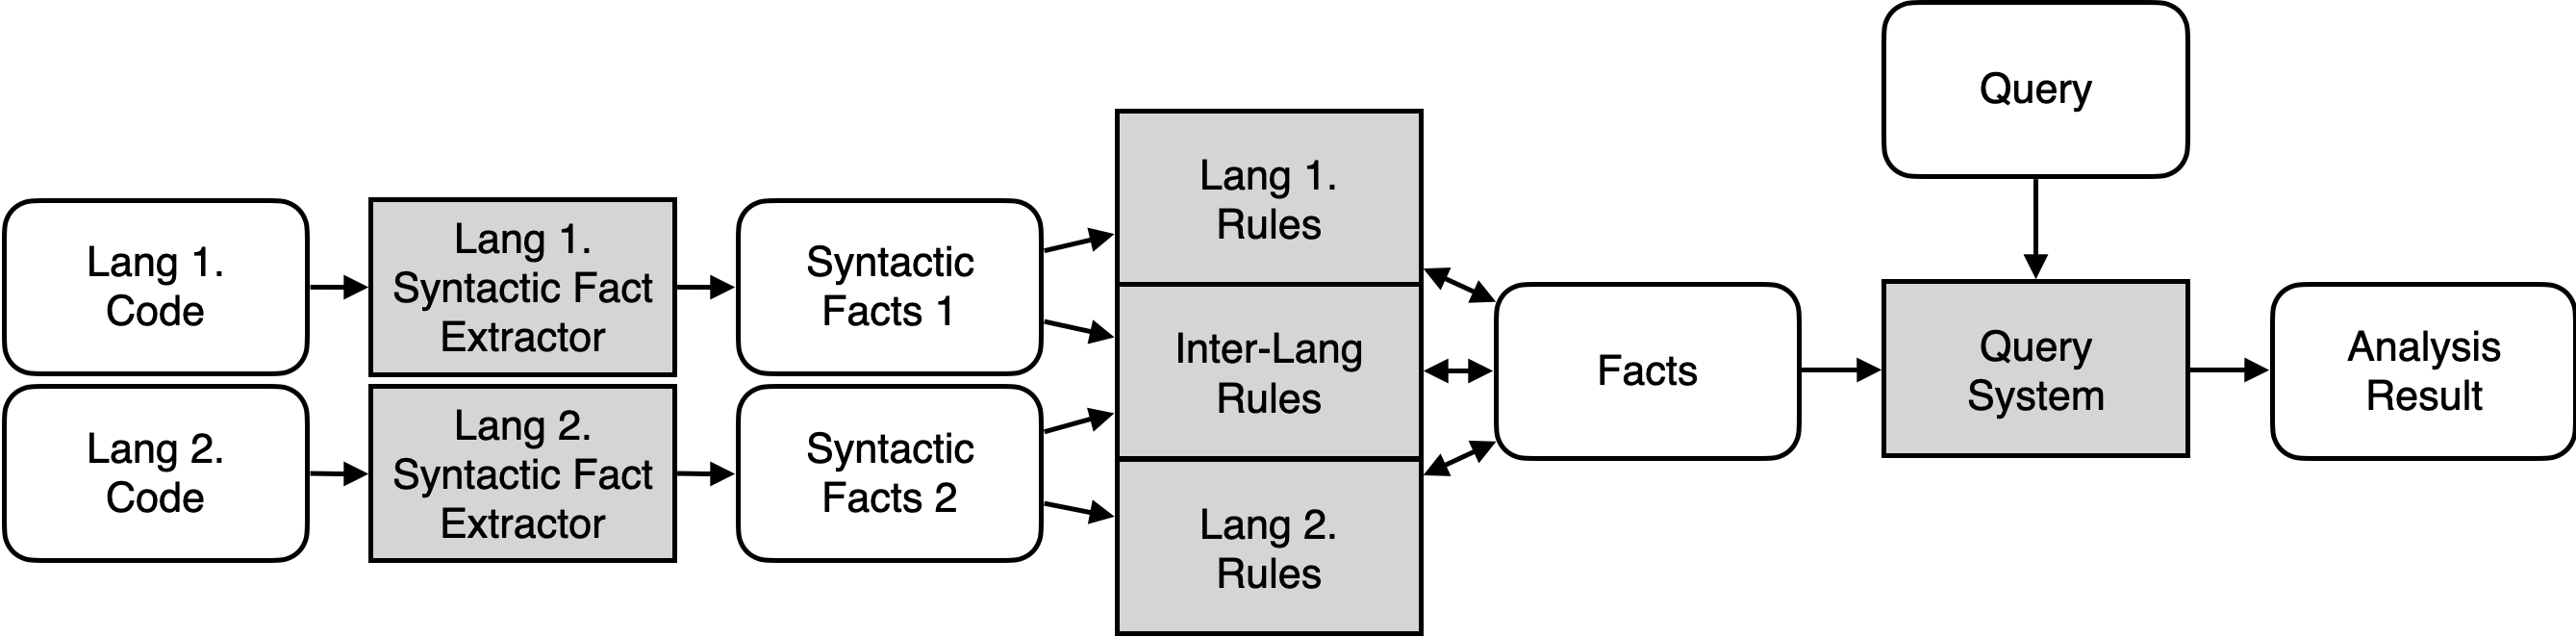
\includegraphics[width=0.47\textwidth]{img/ov2.png}
  \caption{Declarative analysis for multilingual programs}
  \label{fig:ov2}
%\vspace*{-.5em}
\end{figure}

\subsection{Overview}
Figure~\ref{fig:ov2} illustrates how we support multilingual analysis in a
declarative style in the case of two languages as an example. The declarative
language engine now gets two sets of syntactic facts extracted from different
languages. In addition, new language-interoperation rules are defined on top of
the original language-specific rules from different languages to take the
interoperation semantics into account. Then, the same query is performed to get
the actual analysis.

\begin{figure}[t]
  \centering
%  \vspace{2mm}
  \begin{subfigure}[t]{0.23\textwidth}
    \begin{lstlisting}[style=mpython]
import f
def m1():
    f()
def m2():
    pass
m1()
    \end{lstlisting}
    \vspace*{-.5em}
    \caption{Code in language A}
    \label{fig:exam:langA}
  \end{subfigure}
  \begin{subfigure}[t]{0.23\textwidth}
    \begin{lstlisting}[style=mcpp,firstnumber=9]
void f() {
    CallMethod("m2");
}
    \end{lstlisting}
    \vspace*{2.5em}
    \caption{Code in language B}
    \label{fig:exam:langB}
  \end{subfigure}
  \vspace*{-.5em}
  \caption{Multilingual code example written in both A and B}
  \label{fig:exam}
\end{figure}

%Let us consider a multilingual program written in a Python-like language A
%and a C-like language B.
%
%The program in Figure~\ref{fig:exam} has two parts: Figure~\ref{fig:exam}(a)
%shows a method \javacode{m1}, \javacode{m2} in language A, and
%Figure~\ref{fig:exam}(b) shows a function \ccode{f} in language B.  The method
%\javacode{m1} is called from top level of language A, and it calls the the
%function \ccode{f} from language B.  Then, the function \ccode{f} calls back
%the method \javacode{m2} in language A using API function, using the string
%value "m2" to indicate the name of method.

\subsection{Example declarative style analysis}
An example declarative analysis consists of facts and rules, and queries as the
follows:

{\small
\[
  \begin{array}{llll}
    f & ::= & p(\overline{elem | x}) & \text{\sc Fact}\\
    r & ::= & f\ \mbox{:-}\ \overline{\neg^? f} & \text{\sc Rule}\\
    q & ::= & \mbox{?-} \overline{f}\ &  \text{\sc Query}
\end{array}
\]
}

\noindent
The fact $p(\overline{elem | x})$ denotes a relation $p$ between elements
$\overline{elem}$ or variables $\overline{x}$. The elements are primitive
values in the analysis, such as string and integer values.  The rule $f'\
\mbox{:-}\ \overline{\neg^? f}$ denotes that a fact $f'$ is derived from other
facts $\overline{f}$; $f'$ holds if all the facts $f \in \{\overline{\neg^?
f}\}$ hold. The optional prefix negation $\neg$ denotes the negative hold
condition of a fact; A negated fact $\neg f$ holds if the fact $f$ does not
hold. The query ``$\mbox{?-} \overline{f}$'' finds all possible elements that
make all facts in $\overline{f}$ hold if variables in $\overline{f}$ are
replaced with the elements.


\subsection{Declarative call graph construction for monolingual programs}\label{lab:ovmono}


This section describes how the example declarative style analysis constructs call graphs
for two different monolingual code and how we extend the analysis to construct
a unified call graph across languages.
Figure~\ref{fig:exam} shows a multilingual code example written in both (a)
Python-like language {\it A} and (b) C-like language {\it B}. In {\it A}, there
are two functions, {\tt m1} at line~3 and {\tt m2} at line~5. The function {\tt
m1} calls the function {\tt f} in {\it B} via language interoperation between
{\it A} and {\it B}, and the function {\tt m2} does nothing. At line~8 in {\it
A}, the expression {\tt m1()} calls the function {\tt m2} defined at line~3 to
invoke the function {\tt f} in {\it B}.
The {\tt f} function in {\it B} calls the {\tt CallMethod} function with a
string value {\tt "m2"} to invoke the function {\tt m2} in {\it A}, using the
string value argument as the target function name.
%Thus, the code example performs the bidirectional interoperation between {\it
%A} and {\it B}, which calls the function {\tt f} written in {\it A} from {\it
%B} and calls the function {\tt m2} written in {\it B} from {\it A}.


At first, A declarative style analysis creates a database of facts for the
code. Initial facts are just syntactic information extracted from the code.
For example, there are two kinds of facts required for the call graph
construction; {\tt FunctionAt(ln, name)} denotes function definition
information containing its line number {\tt ln} and the function name {\tt
name}, and {\tt CallAt(ln, name)} denotes callsite information
containing the callsite line number {\tt ln} and its target function name {\tt
name}. The initial facts for the Figure~\ref{fig:exam}(a) code are as follows: 

%First, let's consider a hypothetical declarative style analyzer, that supports
%language A.  As a first step, the database of facts are created from the source
%code. THe facts created in this way may contain some syntactic information
%about the source code. For example, we can think of two kinds of facts:
%MethodAt(l, name) which indicates that the method name 'name' is defined at
%line number l, and CallAt(l, name), which indicates there is a call to a method
%named 'name' at line l.  Specifically, the program at Figure~\ref{fig:exam}(a)
%would be transformed into the following facts:

\begin{lstlisting}
FunctionAt(3, "m1")
CallAt(4, "f")
FunctionAt(5, "m2")
CallAt(8, "m1")
\end{lstlisting}

Then, the analysis requires rules for the initial facts to derive new facts
about function call relations. In this example, a kind of facts, {\tt
CallEdge(ln1, ln2)}, denotes a call relation from a callsite at line {\tt ln1}
to a function define at line {\tt ln2}. To derive function call relation facts,
we define a rule as follows: 

%Next, there are rules that derice new facts from the known facts.  In this
%example, we would want to define the rule for generating the facts of
%CallEdge(l1, l2), which indicates there is an call edge from the call
%expression at line l1 to the method definition at line l2. Using the know facts
%of MethodAt and CallAt, we can define the rule like folowing:

\begin{lstlisting}
CallEdge(ln1, ln2) :-
  CallAt(ln1, name),
  FunctionAt(ln2, name)
\end{lstlisting}

%The meaning of this rule is straight forward. Whenever there is a method
%definition and a method call with the sane name, then there is c call edge
%between them.  By applying this rule on top of facts obtained above, we would
%get this new fact:

\noindent
The rule derives a new fact {\tt CallEdge(ln1, ln2)} when a callsite at line
{\tt ln1} has the same target function name as the name of a function defined
at line {\tt ln2}. Therefore, a new fact can be derived from the initial facts
as follows: 

\begin{lstlisting}
CallEdge(7, 3)
\end{lstlisting}

Finally, a query system extracts a set of function call relation facts when we
make a query. Since the rule derives the {\tt CallEdge(7,3)} fact, the
following query produces {\tt (X, Y) $\in$ \{(7, 3)\}} as a result:

%Finally, there is a query system that is used for extracting certain sets of
%facts that meet certain condition. For example, we can simply make a query to
%find every calledge using following query:

\begin{lstlisting}
?- CallEdge(X, Y).
\end{lstlisting}


Otherwise, initial facts for the Figure~\ref{fig:exam}(b) code are as follows: 
%This time, let's look at how the analyzer is extended to support the analysis
%of B. Similar to language A, the first step is to create database. For language
%B, we can have the rules of FunctionAt, CallAt, and Argument as follows:

\begin{lstlisting}
ProcedureAt(9, "f")
CallAt(10, "CallMethod")
Argument(10, 0, "m2")
\end{lstlisting}

\noindent
The kind of facts {\tt ProcedureAt(ln, name)} is identical to {\tt
FunctionAt(ln, name)} for the language {\it A}, but has a different relation
name. The kind of facts {\tt Argument(ln, i, arg)} denotes the syntactic
information of a function call argument, where {\tt ln} is the line number of
the callsite, {\tt i} is the argument position, and {\tt arg} is the argument
value.

Then, we define a slightly different rule to derive a function call relation
from the initial facts as follows: 
%where Argument(l, i, arg) would mean that the function call at line l would
%have arg as the ith argument.  Then we can define the rule for CallEdge in
%similar manner:

\begin{lstlisting}
CallEdge(l1, l2) :-
  CallAt(l1, name),
  ProcedureAt(l2, name)
\end{lstlisting}

\noindent
The rule is language-specific, because it derives the same kind of facts from
different facts for different languages.  The query system produces {\tt (X, Y)
$\in$ \{\}} as a result of the query {\tt ?- CallEdge(X, Y)}, since there are
no facts holding for the rule.
%Note that we can use the same query {\tt ?- CallEdge(X, Y)} to derive function
%call relation facts for both language {\it A} code and {\it B} code, since the
%kind of facts has the same relation name.  

%It is important thing to note here is that, the same name of "CallEdge" is used
%for this rule. The rationale for the developer of analyzers to use the same
%name here, is that the exact same query can be reused. For example, we can use
%the exact same query
%
%?- CallEdge(X, Y).

%to find all possible set of call edges. In this case, the output would be empty
%as the analyzer is not considering the source code from A.

\subsection{Extending declarative call graph construction for multilingual programs}
%So far, we have seen how a declarative analyzer designed for one language can
%be extended to support another language. Now, we can take aadvantage of this

%Again, the first step is to create merged database that can separated into 2
%logical language spaces. In this example, the merged database would look like
%this:

The first step of our extension for multilingual program analysis creates a
merged database that consists of two logical language spaces, {\it A} and {\it
B}. Then, we store initial facts of the Figure~\ref{fig:exam}(a) and (b) to
corresponding language spaces respectively. The following shows the merged
database containing the initial facts, and subscriptions of the facts denote
logical language spaces in which the facts reside: 

\begin{lstlisting}
FunctionAt$_A$(3, "m1")
CallAt$_A$(4, "f")
FunctionAt$_A$(5, "m2")
CallAt$_A$(8, "m1")
ProcedureAt$_B$(9, "f")
CallAt$_B$(10, "CallMethod")
Argument$_B$(10, 0, "m2")
\end{lstlisting}

%Then, the next step is to define the rule for CallEdge.  The new rule will be
%composed of three parts: language-specific rule for A, lanuguage-specific rule
%for B, and language-interoperations rules:

The next step defines a generalized rule to derive function call relation
facts. We define such rules by composing language-specific rules for A,
lanuguage-specific rules for B, and language-interoperation rules as follows:

\begin{lstlisting}
CallEdge(ln1, ln2) :- CallEdge$_A$(ln1, ln2)
CallEdge(ln1, ln2) :- CallEdge$_B$(ln1, ln2)
CallEdge(ln1, ln2) :- CallEdge$_{AB}$(ln1, ln2)
CallEdge(ln1, ln2) :- CallEdge$_{BA}$(ln1, ln2)
\end{lstlisting}

%For language-specific rules for CallEdge\_A and CallEdge\_B can be defined same
%as before.  For language-interoperation rule, both call from A to B and B to A
%should be considered. In our example language, call from A to B is similar to
%normal method call from B to B, so the rule for CallEdge\_AB can be defined in
%similar way:

\noindent 
We slightly modify the language-specific rules for {\it A} and {\it B} to
derive the {\tt CallEdge$_A$} and {\tt CallEdge$_B$}:

\begin{tabular}{ll}
  {\begin{lstlisting}
CallEdge$_A$(ln1, ln2) :-
  CallAt$_A$(ln1, name),
  FunctionAt$_A$(ln2, name)
  \end{lstlisting}} & 
  {\begin{lstlisting}
CallEdge$_B$(l1, l2) :-
  CallAt$_B$(l1, name),
  ProcedureAt$_B$(l2, name)
  \end{lstlisting}}
\end{tabular}

\noindent
In addition, we define additional language-interoperation rules to derive {\tt
CallEdge$_{AB}$} and {\tt CallEdge$_{BA}$}. The kind of facts {\tt
CallEdge$_{AB}$} denotes a function call relation from a function written in
the language {\it A} to a function written in the language {\it B}, and {\tt
CallEdge$_{BA}$} denotes a function call relation in the opposite direction.
Since the function call semantics from {\it A} to {\it B} is the same as the
normal function calls in {\it A}, we define the interoperation rule from {\it
A} to {\it B} as follows: 

%For language-interoperation rule, both call from A to
%B and B to A should be considered. In our example language, call from A to B is
%similar to normal method call from B to B, so the rule for CallEdge\_AB can be
%defined in similar way:

\begin{lstlisting}
CallEdge$_{AB}$(ln1, ln2) :-
  CallAt$_A$(ln1, name),
  ProcedureAt$_B$(ln2, name)
\end{lstlisting}

\noindent
On the other hand, the function call semantics from {\it B} to {\it A} is
different from the normal function calls in {\it B}. The language {\it B} calls
a function written in {\it A} by calling an interoperation API function {\tt
CallMethod} with a target function name as the first argument. Thus, we define
the interoperation rule from {\it B} to {\it A} as follows: 

%For the rule for CallEdge\_BA, the situation is a bit trickier.  Since the
%method call is done via an api function call, we weill have to consider this
%semantics.

\begin{lstlisting}
CallEdge$_{BA}$(ln1, ln2) :-
  CallAt$_B$(ln1, "CallMethod"),
  Argument$_B$(ln1, 0, name),
  FunctionAt$_A$(ln2, name)
\end{lstlisting}

%After fully defining the rule for CallEdge, then we can reuse the query system
%just as before to findout every possible calledge:
%
%?- CallEdge(X, Y).
%which will give us the output, (X, Y) = (7, 3), (4, 9), (10, 5)

Finally, when we make the same query {\tt ?- CallEdge(X, Y)}, the query system
produces functions call relations as {\tt (X, Y) $\in$ \{(7, 3), (4, 9), (10,
5)\}}, which include not only call relations among functions written in a
language, but also interopreation function call relations. 

This simple example shows what our extension for multilingual program analysis
requires. Our extension reuses most of parts of an existing declarative style
analysis with slight modifications. Because the modifications of a database and
language-specific rules is trivial, we can fully automate the modification
process.  The only manual part in our extension is to define additional
language-interoperation rules. We detail a proof-of-concept extension of CodeQL
for Java-C and Python-C programs in Section~\ref{sec:impl}.

%It is interesting to see what is the only required task for this extension.
%Most of the parts in original analyzers is reused, and the only requirements
%are the additional language-interoperation rules, in this case,
%language-interoperation rules for CallEdge\_AB and CallEdge\_BA. Rest of the
%part can be constructed in automated way.

%Starting?\tikzmark{}? from the next section, we formally present our approach to extend the
%analyzer targeting multiple lanugaes to support multilingual analysis, specific
%implementation details on extedning CodeQL to support Java-C programs and
%Python-C programs, and demonstrate our experimental result with the
%proof-of-concept implementation.
